\newcommand{\pluginName}{Point Function 2D}
\newcommand{\pluginVersion}{1.0.0}

\input{../../../DocumentationTemplate/TemplateL3}

\section{Introduction}
The \emph{Point Function 2D} plug-in allows you to define a bi-dimensional function defined by given points. The missing data is, then, generated by interpolation or extrapolation.

You have 3 types of interpolation available:
\begin{itemize}
\item Bi-linear interpolation
\item zero order interpolation
\item left zero order interpolation
\end{itemize}

The extrapolation is supported by constant value (the value at the nearest available data point is replicated).

\section{How to use the plug-in}
In the Fairmat user interface when adding a new parameter \& functions.
you will find the additional option \emph{2D Function defined by value interpolation} under functions.
You will then be shown a window similar to the one used to define the 1D version of this plug-in, but differently than that one, you will be given the freedom to define as many columns and as many rows as you wish. (See also Figure~\ref{fig.PFunction2DGUI})

\begin{figure}[h]
\begin{center}
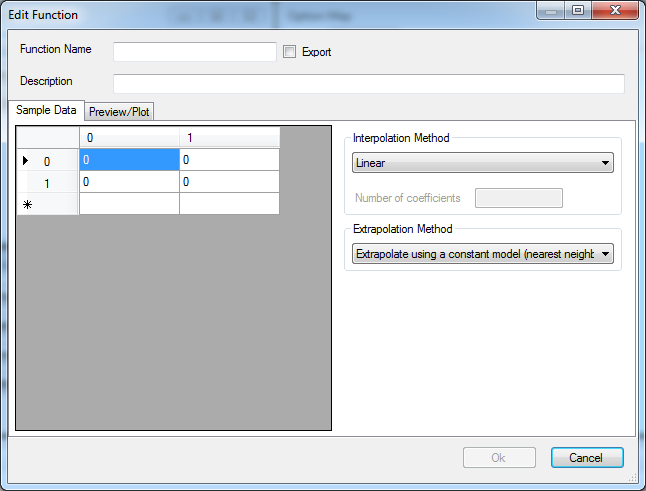
\includegraphics[width=0.48\textwidth]{./images/PFunction2DEdit.png}
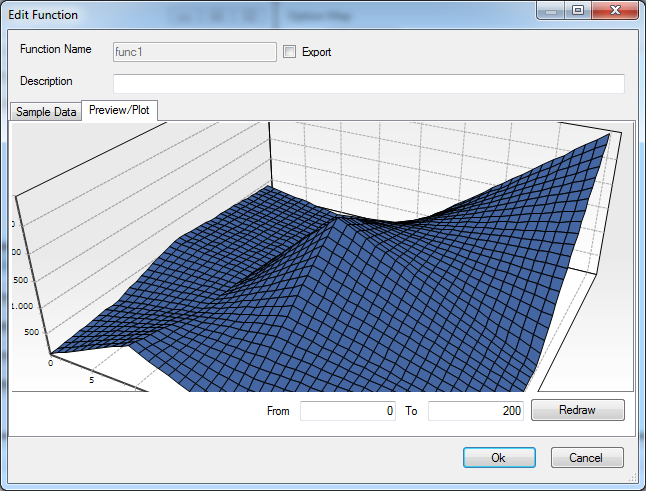
\includegraphics[width=0.48\textwidth]{./images/PFunction2DPreview.png}
\caption{Point Function 2D GUI: input parameters editor and preview.}
\label{fig.PFunction2DGUI}
\end{center}
\end{figure}

In order to give values to coordinates you can double click on the row/column header, this way you will be shown 
a window allowing to fill them in (See also Figure~\ref{fig.PFunction2DColumnEdit}), additionally you can add/remove columns by right clicking on the columns headers and selecting one of the contextual options allowing to remove them or insert then before or after the current one. The same identical procedure can be done with rows.

As for filling the data points, you'll just have to fill the single cells which will be there when creating rows or columns.

\begin{figure}[h]
\begin{center}
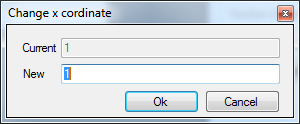
\includegraphics[width=0.48\textwidth]{./images/PFunction2DColumnEdit.png}
\caption{Editing cordinate values.}
\label{fig.PFunction2DColumnEdit}
\end{center}
\end{figure}

You are given the freedom to use any formula for coordinates and point values, but remember that during evaluation the coordinates must always increase while going from left to right and from up to bottom, or you'll get an error during evaluation.

Finally on the right of the window you can choose the interpolation and extrapolation methods you want to apply to the function evaluation.

\end{document}
